\documentclass[../../main.tex]{subfiles}

\begin{document}

\subsubsection{Introduction}

In this iteration I will start working on the frontend, or the client application. The client
application will talk to the backend service I created in the previous iteration and will
provide the client with an intuitive user interface through which they can interact with the
backend service and by extension the database connected to it.

\noindent \\ The two applications, as I mentioned in the first iteration's introduction,
will communicate using GraphQL. The client application itself will make use of
React Native and Expo.

\noindent \\ React Native is an open-source user interface (UI) framework created by
Facebook which allows developers to easily write native applications using
the high-level JavaScript and TypeScript languages. This is opposed to the conventional method
of writing applications for these platforms where different apps would need to be programmed
in different languages for different systems (eg. Android, iOS). React Native allows code to
be written once in a high level language and subsequently executed on multiple
platforms without modification.

\noindent \\ Expo is an open-source SDK (\textbf{S}oftware \textbf{D}evelopment \textbf{K}it) designed to allow high-level code, such as code
written for React Native, to access low-level platform-specific features, such as a devices' camera.
It acts as an \textbf{abstraction layer} providing a generic interface to access such features.

\begin{comment}
\noindent \\ Therefore, the first task to do is to initialise an Expo project and install
our dependencies, notably the Apollo GraphQL client.\
\end{comment}

\subsubsection{Prototyping using the 'Expo Go' application}

Expo Go is a sandbox used to execute an Expo project without having to build it to a native application.
Expo Go can be installed from app-stores and connects to a server located
on another machine (Started using \lstinline{expo start}) which contains the source code.

\noindent \\ JavaScript is an interpreted language, but platform-specific components of both
the Expo SDK and React Native are written in a compiled language such as Java (Android) or Swift (iOS).
Expo Go works by providing a barebones application with the required native code already compiled,
so a server can simply host the remaining interpreted JavaScript code.

\noindent \\ For this iteration, I will use Expo Go for quick prototyping.
However, it is important to note that Expo Go does have it's limitations.
Namely, any dependencies requiring additional native code will not work in Expo Go.
I will need to be aware of this during development of this and future frontend iterations.

\subsubsection{Creating an Expo project}

There are two requirements to consider before creating an Expo project.
The first requirement is to install Node.js, the second to decide which Expo SDK version
to use. Node.js is a portable JavaScript runtime which is used to execute the tools necessary
to create an Expo project.

\noindent \\ Expo Go supports the last three Expo SDK releases.
I have chosen to use the latest SDK at the time of writing, SDK 50.
I chose this version as it introduces a new version of a core expo feature,
\lstinline{expo-router} version 3.

\noindent \\ To create an Expo project, assuming Node.js is installed, open a terminal and type:

% TODO: move to minted? 
% https://tex.stackexchange.com/questions/89276/insert-bash-code-with-coloration-into-my-latex-report
\begin{lstlisting}[language=bash]
    [james@linux cs-coursework]$ npx create-expo-app@latest fosscat-frontend --template tabs@50
\end{lstlisting}

\noindent Wait for the command to finish, and you will have the following output:

\begin{lstlisting}[language=bash]
Need to install the following packages:
create-expo-app@2.3.1
Ok to proceed? (y) y
> Downloaded and extracted project files.
> Your project is ready!

To run your project, navigate to the directory and run one of the following npm commands.

- cd fosscat-frontend
- npm run android
- npm run ios
- npm run web
\end{lstlisting}

\noindent \\ \lstinline{npx} is a Node.js command that allows us to execute the contents of a package,
installing the package if was not already available. We are executing the package \lstinline{create-expo-app}
with the argument \lstinline{fosscat-frontent} as the package name.
We are also making use of a \lstinline{expo-router} template, namely the "tabbed" template.
This means that create-expo-app will also generate boilerplate code for \lstinline{expo-router},
such as an initial home page (or route).

\noindent \\ This command sets up and creates an Expo project, including installing dependencies such as
React, React Native and TypeScript.

% Dummy env to escape wrapfig
\begin{dummyenv}

  \begin{wrapfigure}{r}{0.4\textwidth}
    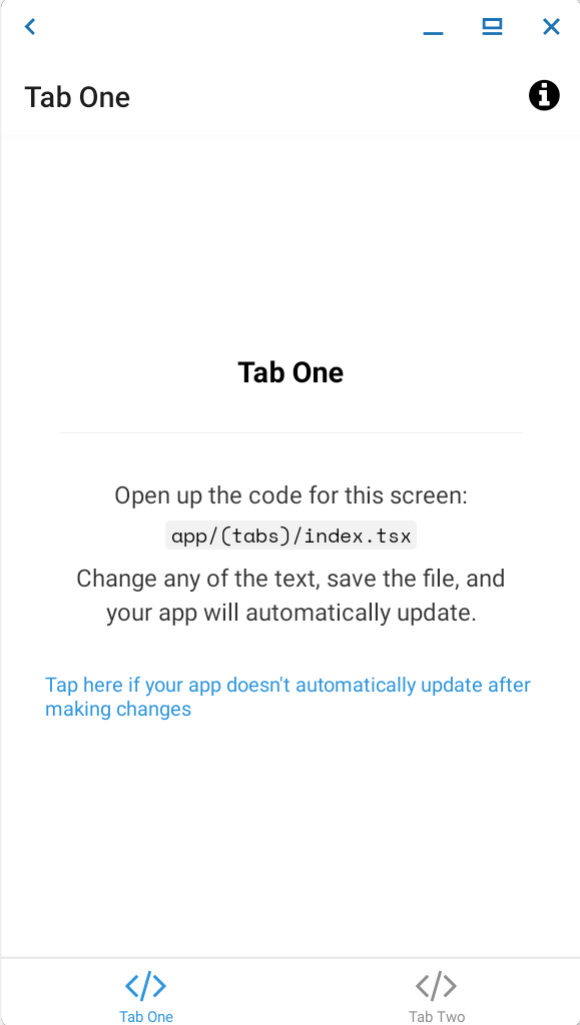
\includegraphics[width=\linewidth, frame]{implementation/second iteration/ca5b6d244e53f298ad7fe0d304d3591698032a39.png}
    \label{fig:wrapfig}
  \end{wrapfigure}

  \noindent \\ We can preview our changes in real-time on an iOS or Android device by running \lstinline{npx expo start}.
  If we run this command now we can see the generated boilerplate code in action on the right:

  \noindent \\ Below is the generated function that renders this page.

  \begin{lstlisting}[language=typescript, breaklines=false]
      // Imports omitted

      export default function TabOneScreen() {
        return (
          <View style={styles.container}>
            <Text style={styles.title}>Tab One</Text>
            <View
              style={styles.separator}
              lightColor="#eee"
              darkColor="rgba(255,255,255,0.1)"
            />
            <EditScreenInfo path="app/(tabs)/index.tsx" />
          </View>
        );
      }

      // Styling omitted
    \end{lstlisting}

  \noindent \\ React syntax is remarkably similar to that of HTML,
  but with two key differences:

\end{dummyenv}

\begin{enumerate}
  \item React has custom elements or "components" (eg. \lstinline{View})
  \item React can have inline JavaScript/Typescript by using curly brackets, eg.\\
        \lstinline[language=typescript]|<Button onClick={/* js/ts code here */ } />|
\end{enumerate}

\subsubsection{Integrating the Apollo GraphQL client for backend communication}

As mentioned previously, the client (frontend component) and server (backend component)
will communicate using GraphQL. \textbf{Apollo Client} is a GraphQL client designed for use with
React and React Native. It can be installed using
\lstinline[language=bash]{npm install @apollo/client graphql}.

\subparagraph{Configuring Apollo Client to talk to the backend component\\}

% SKIP for now: (frontend/metro):  Allow mjs files to be imported to make graphql package work

\noindent \\ Now that Apollo has been installed, I needed to set it up to connect to the backend.

In the design section, I planned this using React Hooks and React Context.

% ADD TO DESIGN

\end{document}